\section{Spécification du Système}
Cette partie du cahier de charge présentera les trois axes principaux du développement de ifind.
\begin{itemize}
 \item Architecture du système.
 \item Charges du système.
 \item Modèles dy système.
\end{itemize}

\subsection{Architecture du Système}
Ce paragraphe présente un point du vue haut niveau de l'architecture préconisée du système et la distribution de fonctionnalités à travers 
les modules du système.

Notre système se compose de trois sous-systèmes :
\begin{itemize}
 \item Moteur de recherche : Architecture Model View Controler
 \item Moteur d'indexation : Deamon
 \item Base de donnée indexée : Architecture en couche : PostgreSQL
\end{itemize}

\subsubsection{Architecture du Moteur de recherche}
Le moteur de recherche (MR) communique avec la base d'indexation (BI) par l'intermédiaire d'un flux XML au travers d'une Socket.
Le flux XML envoyé par le MR est associé à un identifiant, qui permet de savoir à quelle requête est associée quelle réponse.
L'envoi respecte la DTD (voir annexe).

\paragraph{BNF}
Nous avons défini une syntaxe et à fortiori, une grammaire sous forme BNF.

Grammaire (BNF) :\\
% \begin{tabular}{r c l}
% query &$\rightarrow$ & word { -or word } [options]\\
% query &$\rightarrow$ & word { word } [options] \\
% 	 
% options&$\rightarrow$ &-e word {word}\\
% word   &$\rightarrow$ &char*\\
% char   &$\rightarrow$ & [a-z A-Z 0-9 à é è ë ä ù ï ç]\\ 
% \end{tabular}

\begin{tabular}{p{1.5cm} p{0.5cm} p{9cm} }
& & \\
\textbf{char} & $\equiv$ & [:alnum:]\\
\textbf{word} & $\equiv$ & $\textbf{char}^+$\\
\textit{query} & ::= & \textbf{word} \textit{\{} \textbf{-or} \textbf{word} \textit{\}} \textit{[} \textit{options} \textit{]}\\
& | & \textbf{word} \textit{\{} \textbf{word} \textit{\}} \textit{[} \textit{options} \textit{]}\\
\textit{options} & ::= & \textbf{-e} \textbf{word} \textit{\{} \textbf{word} \textit{\}}\\
\end{tabular}

Par la suite, nous avons défini plusieurs types abstraits de données permettant de modéliser la grammaire.
Un type a forcément une ou plusieurs opérations de construction. 
Chaque type peut présenter des fonctions d'accès et de test ainsi que des constantes.

\paragraph{Type de données abstraites}
En effet, nous avons définit 6 types tels que :

\begin{tabular}{r l}
%\textbf{Type : operateur} & \\
%constantes :& plus, OR et Exclu : operateur
% note (isabelle) La présence des types [conj] et [disj] rend la constante [operateur] inutile.

\textbf{Type : requête} & \\
_construction :& cons-requete-word : word $\rightarrow$ requête\\
& cons-requete-word-options : word * options $\rightarrow$ requête\\ 
& cons-requete-conj : conj $\rightarrow$ requête\\
& cons-requete-conj-options : conj * options $\rightarrow$ requête\\
& cons-requete-disj : disj $\rightarrow$ requête\\
& cons-requete-disj-options : disj * options $\rightarrow$ requête\\
_test :& est-word : requête $\rightarrow$ bool\\
& est-conj : requête $\rightarrow$ bool\\
& est-disj : requête $\rightarrow$ bool\\
& a-options : requête $\rightarrow$ bool\\
% est-valide : requête $\rightarrow$ bool\\
% note (isabelle) une requête qui est construite est par définition valide (sauf erreur de ma part), donc ce test est inutile.
_accès :& get-word : requête $\rightarrow$ word\\
& get-conj : requête $\rightarrow$ conj\\
& get-disj : requête $\rightarrow$ disj\\
& get-options : requête $\rightarrow$ options\\
\end{tabular}

\paragraph{}
On garde get-conj() si est conj : get-word() puis recherche conjonction et
get-disj() si est disj : get-word() puis recherche disjonction.
\paragraph{}

\begin{tabular}{r l}
\textbf{Type : conj} &\\
_construction :& cons-conj : word * conj $\rightarrow$ conj\\
& cons-conj-simple : word * word $\rightarrow$ conj\\
_test :& est-conj : conj $\rightarrow$ bool\\
_accès :& get-head : conj $\rightarrow$ word\\
& get-tail : conj $\rightarrow$ conj\\
& \\

\textbf{Type : disj}&\\
_construction :& cons-disj : word * disj $\rightarrow$ disj\\
& cons-disj-simple : word * word $\rightarrow$ disj\\
& accès : getDisj()\\
& \\

\textbf{Type : word}&\\ 
_construction :& cons_word : string $\rightarrow$ word\\
_accès :& get-word : word $\rightarrow$ string\\
& \\

\textbf{Type : options}&\\
_construction :& cons-options : word $\rightarrow$ options\\
& cons-options-simple : word * word $\rightarrow$ options\\
_test :& est-options : options $\rightarrow$ bool\\
_accès :& get-head : options $\rightarrow$ word\\
& get-tail : options $\rightarrow$ options
\end{tabular}


Model :

View : GUI

Controler : search-engine-core
\begin{center}
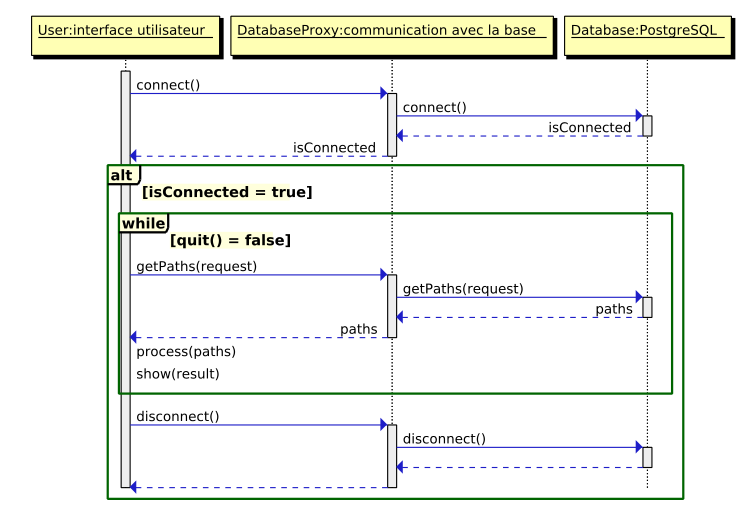
\includegraphics[scale=0.5]{seqmrbi.png}
\end{center}


\subsubsection{Architecture du moteur d'indexation}
Le moteur d'indexation se compose de deux instances.\\
La première est lancée uniquement lorsqu'il faut entièrement créer l'index (lors de l'installation, par exemple).\\
La deuxième, le démon, communique en permanence avec la base d'indexation afin de lui envoyer
les différents évènements qui ont eu lieu à l'intérieur du corpus et qui doivent être indexés.
L'envoi se fait par l'intermédiaire d'un flux XML au travers d'une Socket. L'envoi respecte la DTD (voir annexe)
établie par les chefs de projets pendant les réunions.

\subsubsection{Architecture de la base d'indexation}
La base d'indexation est une base de donnée PostgreSQL, en un premier temps, qui permettra au moteur de recherche 
de retrouver ce qu'il cherche.

\begin{center}
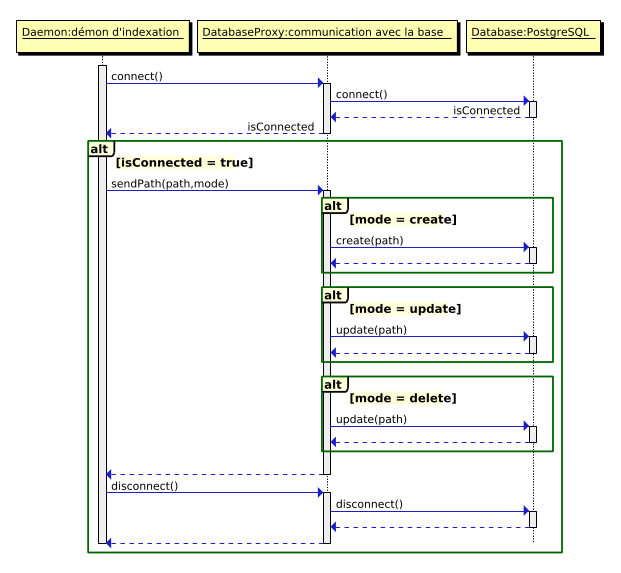
\includegraphics[scale=0.5]{seqdbi.png}
\end{center}

Le modèle conceptuel de données (MCD) de la base de données est le suivant :
\begin{center}
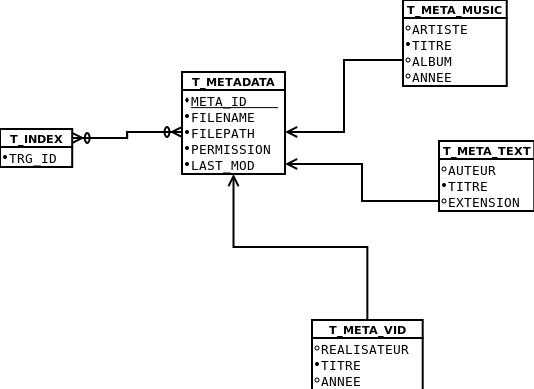
\includegraphics[scale=0.7]{mcd.png}
\end{center}


\subsection{Charges du Système}
Ce paragraphe décrit les charges fonctionnelles du système en détail et d'autres charges non fonctionnelles : 
\begin{itemize}
 \item interface
 \item autres...
\end{itemize}

\subsection{Modèles du système}
Ce paragraphe décrit les divers modèles du système ainsi que leurs relations entre composantes du système et de son environnement.

\subsubsection{Modèle de communication}
Le base d'indexation écoute sur deux ports différents, un pour la communication avec le moteur d'indexation, 
et un pour la communication avec le moteur de recherche.

\paragraph{Communication avec le moteur d'indexation}
La base d'indexation (BI) attend qu'un moteur d'indexation (MI) se connecte sur le port 40000. Lorsque la connexion est établie, 
la BI lit le flux XML envoyé par le MI. La connexion entre le MI et la BI n'est fermée que lorsque l'un des deux modules
est fermé.

\paragraph{Communication avec le moteur de recherche}
La base d'indexation (BI) attend qu'un moteur de recherche (MR) se connecte sur le port 30000. Lorsque la connexion est établie,
la BI lit le flux XML envoyé par le MR. La BI génère une réponse au flux et la renvoie au MR, via le port 30000 sous forme de XML.
